% Marco Teórico.tex

\chapter{Marco Teórico}
\label{c2} 




\section{Evolución del sistema eléctrico en Chile}\label{c21}

El sistema eléctrico en Chile ha experimentado una serie de cambios significativos desde su diseño original hace cuatro décadas. Estos cambios han sido impulsados por una combinación de factores, incluyendo la liberalización del mercado, la introducción de nuevas tecnologías y la creciente preocupación por el medio ambiente.
\vspace{2.5mm}

En la década de 1980, Chile fue uno de los primeros países en el mundo en liberalizar su sector eléctrico. Esta liberalización se llevó a cabo en el marco de una serie de reformas económicas más amplias que buscaban reducir el papel del estado en la economía y promover la competencia y la eficiencia del mercado. Como resultado de estas reformas, se creó un mercado mayorista de electricidad en el que las empresas generadoras venden su electricidad a las empresas distribuidoras a través de un sistema de subastas competitivas.
\vspace{2.5mm}

En los primeros años del mercado mayorista, la generación de electricidad en Chile estaba dominada por un pequeño número de grandes centrales hidroeléctricas y térmicas. Sin embargo, a lo largo de los años, la matriz energética del país ha evolucionado para incluir una mayor diversidad de fuentes de energía. En particular, ha habido un crecimiento significativo en la generación de energía a partir de fuentes renovables, como la energía eólica y solar.
\vspace{2.5mm}

Este cambio en la matriz energética ha sido impulsado en parte por la introducción de políticas gubernamentales que promueven el uso de energías renovables. Por ejemplo, en 2008, el gobierno chileno introdujo una ley que requiere que una cierta proporción de la electricidad vendida por las empresas distribuidoras provenga de fuentes renovables. Esta proporción ha ido aumentando con el tiempo, y se espera que continúe aumentando en el futuro.
\vspace{2.5mm}

Además de la diversificación de la matriz energética, también ha habido cambios significativos en la estructura del mercado eléctrico. En particular, ha habido un movimiento hacia una mayor integración de los mercados eléctricos regionales. En 2017, los dos principales sistemas eléctricos de Chile, el Sistema Interconectado Central (SIC) y el Sistema Interconectado del Norte Grande (SING), se fusionaron para formar el Sistema Eléctrico Nacional (SEN). Esta fusión ha permitido una mayor eficiencia en la operación del sistema eléctrico y ha facilitado la integración de las energías renovables.
\vspace{2.5mm}

A pesar de estos cambios, el sistema eléctrico de Chile todavía enfrenta una serie de desafíos. Uno de los principales desafíos es la necesidad de equilibrar la creciente demanda de electricidad con la necesidad de reducir las emisiones de gases de efecto invernadero. Otro desafío es la necesidad de garantizar la seguridad del suministro de electricidad en un contexto de creciente variabilidad y incertidumbre en la generación de energía renovable.
\vspace{2.5mm}


Según \citeB{serra_chiles_2022}, algunos de los desafíos clave que enfrenta el sistema eléctrico de Chile incluyen:
\begin{enumerate}
\item 
La integración de las energías renovables: A medida que Chile aumenta su dependencia de las energías renovables, el sistema eléctrico debe adaptarse para manejar la variabilidad y la intermitencia asociadas con estas fuentes de energía. Esto puede requerir inversiones en infraestructura de red, así como el desarrollo de mercados de capacidad y servicios auxiliares para garantizar la estabilidad del sistema.
\item 
La descarbonización del sistema eléctrico: Chile se ha comprometido a reducir sus emisiones de gases de efecto invernadero y a descarbonizar su sistema eléctrico. Esto implica un cambio significativo en la matriz energética del país, con un alejamiento de los combustibles fósiles y un aumento en la generación de energía renovable. Este proceso de descarbonización también requerirá cambios en la regulación y la política energética.
\item 
La eficiencia del mercado eléctrico: Aunque el mercado eléctrico de Chile ha funcionado bien en general, existen áreas en las que se puede mejorar la eficiencia. Por ejemplo, el autor señala que el sistema actual de precios de la electricidad, que se basa en el costo marginal de la generación, puede no reflejar adecuadamente los costos totales de la generación de electricidad. Esto puede llevar a distorsiones en las señales de precio y a una asignación ineficiente de los recursos.
\item 
La equidad en el acceso a la electricidad: Aunque la cobertura eléctrica en Chile es alta, existen diferencias en el acceso a la electricidad entre las diferentes regiones y grupos socioeconómicos. Garantizar un acceso equitativo a la electricidad es un desafío importante, especialmente a medida que el país se mueve hacia una matriz energética más sostenible.
\end{enumerate}

Estos desafíos son complejos y requieren una combinación de soluciones técnicas, regulatorias y políticas. Sin embargo, a medida que Chile continúa su transición hacia una matriz energética más limpia y sostenible, estos desafíos también representan oportunidades para innovar y mejorar el sistema eléctrico del país.\vspace{2.5mm}

El año 2023 se presenta como un punto de inflexión crucial para la transición energética en Chile. Los expertos sostienen que este año, el país debe enfrentar varios desafíos que implica tener una matriz más limpia, como una mejor gobernanza y coordinación entre organismos, un marco regulatorio más afinado y un sistema tarifario atractivo para el desarrollo de esta industria, al tiempo que debe asegurarse el desarrollo de las Energías Renovables No Convencionales (ERNC) de las próximas dos décadas.\vspace{2.5mm}

Se han dado pasos importantes en este sentido, como la promoción del hidrógeno verde, impulsada mediante una estrategia nacional, y la Estrategia Nacional de Electromovilidad, que contempla el ingreso a tramitación del proyecto de ley de transición energética, que busca promover el almacenamiento de energía eléctrica y la electromovilidad. Estos esfuerzos han contribuido a posicionar a Chile como uno de los países que lideran la transición energética en Latinoamérica. Por ejemplo, el año pasado, la energía solar y eólica superaron al carbón en la generación de electricidad en un período de 12 meses, según el Coordinador Eléctrico Nacional (CEN) y la Comisión Nacional de Energía. El 29\% de la generación anual provino de fuentes de energía solar y eólica, y el 27\% del carbón.\vspace{2.5mm}

Sin embargo, a pesar de los avances significativos, los especialistas coinciden en que todavía queda mucho camino por recorrer. El país requiere de inversión, actualización de las normativas, acuerdos público-privados y también diálogos ciudadanos para solucionar algunos cuellos de botella como, por ejemplo, mejorar el sistema de transmisión, sistemas de almacenamiento y lograr la escalabilidad de las nuevas tecnologías.

\section{Dificultades en la transición hacia energías renovables}\label{c22}

La transición hacia una matriz energética basada en fuentes renovables es un objetivo ambicioso y necesario para muchos países, incluido Chile. Sin embargo, este proceso no está exento de desafíos y obstáculos que pueden ralentizar o complicar su implementación.\vspace{2.5mm}

Empresas de energía renovable, principalmente solares, han invertido en Chile más de 5.000 millones de euros en proyectos de esta naturaleza.\footnote{Ver artículo en \href{{https://elpais.com/chile/2023-06-20/el-plan-del-ministro-de-energia-de-gabriel-boric-para-aliviar-a-las-renovables.html}}{El País}} A pesar de este impulso, la transición ha enfrentado problemas significativos. Dos generadoras notables, María Elena Solar e Ibereólica Cabo Leones II, se declararon en quiebra, y al menos nueve empresas del sector expresaron su inquietud sobre la posibilidad de que más compañías enfrenten insolvencia.\vspace{2.5mm}

El atraso en la construcción de líneas de transmisión ha provocado que compañías que inyectan energía al sistema en el norte del país lo hagan a precio cero, pero luego deben retirar en la zona centro-sur a precios mucho mayores. Esta situación ha desestabilizado su capacidad financiera, poniendo en riesgo la viabilidad de muchos proyectos. Además, el alto precio de los combustibles fósiles, que compiten con las renovables, también genera distorsiones en los costos. En 2023, más del 35\% de la energía renovable se ha valorizado a un precio cero, evidenciando una crisis en el modelo de tarificación de la generación eléctrica.\vspace{2.5mm}

El Gobierno chileno, consciente de estos desafíos, ha propuesto medidas para abordarlos. Una de las iniciativas más destacadas es el proyecto de ley de Transición Energética, que busca fortalecer el sistema de transmisión, eliminar burocracia en la construcción de infraestructuras y resolver los cuellos de botella. Una medida significativa es la propuesta de eliminar la figura del Coordinador Eléctrico, permitiendo que las empresas establezcan una relación directa con la Comisión Nacional de Energía.\vspace{2.5mm}

Las generadoras convencionales han expresado su preocupación, argumentando que las propuestas presentadas por las empresas de energías renovables podrían atacar los fundamentos de diseño del mercado contenidos en la regulación vigente. Es importante señalar que el diseño actual del mercado se definió hace más de 40 años, en un contexto muy diferente al actual, donde la alta penetración de renovables no estaba contemplada.\vspace{2.5mm}

A nivel global, la transición hacia energías renovables es una tendencia creciente. Sin embargo, la experiencia de Chile resalta la importancia de adaptar las regulaciones y estructuras de mercado a las realidades cambiantes de la generación de energía. La experiencia internacional muestra que es esencial revisar y adaptar constantemente las regulaciones para garantizar una transición exitosa.\vspace{2.5mm}

La transición hacia fuentes de energía renovable no es un proceso que pueda realizarse de la noche a la mañana. Es un camino largo y complejo que requiere de adaptaciones constantes, tanto en infraestructura como en regulaciones. Esta complejidad justifica la necesidad de considerar la transición como una variable en el análisis \ref{c31}, ya que su impacto en el sector eléctrico es profundo y duradero.

\begin{comment}
\section{Benchmark sobre los precios de combustibles renovables y no renovables}\label{c23}

El costo del combustible es una consideración importante en cualquier aplicación, ya sea para impulsar un vehículo recreativo o proporcionar energía a una planta de fabricación. \vspace{2.5mm}

\begin{table}[ht]
\scriptsize 
\centering % Centra la tabla
\begin{tabular}{|c|c|c|>{\centering\arraybackslash}p{3cm}|c|}
\hline
\bf{Combustible} & \bf{Tipo}  & \bf{Precio(\$/gallon)} & \bf{Poder Calorífico Inferior (MJ/kg)}
 & \bf{Industrias en las que se utiliza}\\
\hline
Gasolina & No renovable & 2.96 & 44.4 & Transporte, generación eléctrica\\
\hline
Diésel & No renovable & 3.17 & 45.5 & Transporte, generación eléctrica, calefacción\\
\hline
Gas Natural (GNV) & No renovable & 2.11 & 53.9 & Transporte, generación eléctrica\\
\hline
Etanol & No renovable & 2.17 & 26.8 & Transporte, generación eléctrica\\
\hline
Kerosene & No renovable & 3.47 & 43.1 & Calefacción, aviación\\
\hline
Biodiésel & Renovable & 3.08 & 37.3 & Transporte, generación eléctrica\\
\hline
Bioetanol & Renovable & 2.47 & 21.1 & Transporte, generación eléctrica\\
\hline
Biogás & Renovable & 4.27\$/(MMBTU)* & 21.5 & Generación eléctrica, calefacción\\
\hline
Hidrógeno & Renovable & 4.3 (\$/kg) & 141.8 & Transporte, generación eléctrica\\
\hline
\end{tabular}
\begin{itemize}
    \item[a] Fuente: Precio disponible en: \url{https://afdc.energy.gov/fuels/prices.html}
\item[b] Fuente: Poder calorifico disponible en :\url{https://www.iea.org/data-and-statistics} y \url{http://www.fao.org/faostat/en/#data/QC}
\item[c] *Metric Million British Thermal Unit
\item[f] Tabla actualizada al 10/5/2023
\end{itemize}

\end{table}




En el caso del hidrógeno, su precio es medido en kilogramos en lugar de litros o galones.Para convertir el precio del hidrógeno verde de dólares por kilogramo a dólares por galón, es necesario conocer la densidad del hidrógeno y la conversión de unidades. La densidad del hidrógeno es de aproximadamente 0.08988 kg/m³, mientras que un galón equivale a aproximadamente 3.78541 litros. Por lo tanto, un galón de hidrógeno verde pesaría aproximadamente 0.339 kg (0.08988 kg/m³ x 3.78541 L/galón).
\vspace{2.5mm}

Dividiendo el precio por kilogramo (en este caso, 4.3 dólares) por la cantidad de kilogramos en un galón (0.339 kg), se obtiene un precio de aproximadamente 12.68 dólares por galón de hidrógeno verde.
\vspace{2.5mm}


En cuanto a los combustibles renovables que pueden reemplazar a los no renovables en diferentes industrias, aquí están algunas opciones:
\vspace{2.5mm}
\begin{enumerate}
\item 
Transporte: El biodiésel y el bioetanol pueden reemplazar al diésel y la gasolina en vehículos modificados o diseñados para funcionar con estos combustibles. El hidrógeno también es una opción para vehículos de pila de combustible.
\item 
Generación eléctrica: El biogás y el hidrógeno pueden ser utilizados en lugar de combustibles fósiles como el carbón, el gas natural y el diésel en plantas de generación eléctrica.
\item 
Calefacción: El biogás puede ser utilizado en lugar del gas natural y el kerosene para calefacción en hogares e industrias.
\item 
Industria: El biogás y el hidrógeno pueden reemplazar al gas natural y al carbón en procesos industriales que requieren calor o energía.
\vspace{2.5mm}
\end{enumerate}

Un combustible con un poder calorífico inferior (PCI) más alto se considera más eficiente en términos de aprovechamiento energético. El PCI se refiere a la cantidad de calor liberado cuando un combustible se quema por completo, excluyendo el calor latente del vapor de agua producido durante la combustión.
\vspace{2.5mm}

Cuando un combustible tiene un PCI más alto, significa que se libera más energía térmica por unidad de masa al quemarlo. Esto implica que se puede obtener más calor útil de dicho combustible en comparación con otros combustibles con un PCI más bajo.
\vspace{2.5mm}

El PCI es esencial para maximizar la eficiencia energética, reducir costos y promover la sostenibilidad en diversas industrias. En el transporte, un alto PCI significa mayor eficiencia y menor costo operativo, al ofrecer más energía por unidad de combustible. En la generación eléctrica, un alto PCI implica mayor producción de energía por combustible consumido, optimizando la eficiencia y los costos. Para la calefacción, un alto PCI garantiza una mayor cantidad de calor por combustible, siendo más eficiente y económico.
\vspace{2.5mm}

El gas natural es una fuente de energía fósil, pero es más limpia que la gasolina y el diésel, y su precio es más estable que el de los combustibles líquidos. Además, el gas natural vehicular (GNV) puede ser una fuente de energía renovable si se produce a partir de fuentes renovables, como el biogás.
\vspace{2.5mm}

Por otro lado, el hidrógeno es un combustible renovable que se puede producir a partir de fuentes de energía renovable, como la energía solar y eólica. Aunque el hidrógeno es más caro que los combustibles fósiles, su precio está disminuyendo a medida que se desarrollan nuevas tecnologías para su producción y almacenamiento. Se puede observar en la tabla que el poder calorífico inferior del hidrógeno es, por lejos, el más alto.
\vspace{2.5mm}
\end{comment}

\section{Teoría de juegos}\label{c26}

La teoría de juegos es una rama de las matemáticas que se utiliza para analizar situaciones estratégicas, donde el resultado para un individuo o agente depende tanto de sus propias decisiones como de las decisiones tomadas por otros. Esta teoría tiene aplicaciones en una variedad de campos, incluyendo economía, ciencias políticas, psicología, biología , ciencias de la computación, entre otros.
\vspace{2.5mm}

En términos generales, la teoría de juegos se utiliza para estudiar cómo los agentes toman decisiones en diferentes contextos y cómo estas decisiones están influenciadas por una variedad de factores. Estos factores pueden incluir las acciones de otros agentes, las reglas del juego o sistema en cuestión, y la información disponible para el agente en el momento de la decisión.
\vspace{2.5mm}

Existen dos tipos principales de juegos en la teoría de juegos: cooperativos y no cooperativos. En los juegos cooperativos, los jugadores pueden formar coaliciones y hacer acuerdos vinculantes, mientras que en los juegos no cooperativos, cada jugador actúa de manera independiente para maximizar su propio beneficio.
\vspace{2.5mm}

Un ejemplo clásico de la teoría de juegos en acción es el dilema del prisionero, un juego no cooperativo en el que dos individuos son arrestados y acusados de un crimen. Cada prisionero tiene la opción de traicionar al otro (confesar) o permanecer en silencio. El resultado para cada prisionero depende tanto de su propia decisión como de la decisión del otro prisionero.
\vspace{2.5mm}

En el campo de la economía, la teoría de juegos se utiliza para modelar una variedad de situaciones, desde subastas hasta negociaciones de contratos. Un ejemplo notable es el estudio de la Organización de Países Exportadores de Petróleo (OPEP), donde los países miembros deben decidir cuánto petróleo producir y a qué precio venderlo. La decisión de cada país afecta tanto a su propio beneficio como al de los demás miembros de la OPEP.
\vspace{2.5mm}

\subsection{Juego estático con información completa o perfecta}\label{C261}
En los juegos estáticos con información completa o perfecta, cada agente tiene un conjunto de estrategias disponibles y toma su decisión de manera simultánea, sin tener conocimiento de las decisiones que están tomando los demás agentes en ese mismo momento. Se asume que todos los agentes son racionales y buscan maximizar su propia utilidad, y que cada agente tiene conocimiento completo de las funciones de utilidad de los demás agentes. En otras palabras, cada agente sabe qué es lo que los demás valoran y cómo toman sus decisiones.
\vspace{2.5mm}

Un supuesto clave en este tipo de juegos es que los agentes tienen información completa sobre el juego y sus participantes. Esto significa que conocen todas las estrategias posibles, los pagos asociados con cada combinación de estrategias, y las funciones de utilidad de los demás agentes. En la práctica, este supuesto puede no ser realista en muchas situaciones, pero proporciona una base útil para el análisis.
\vspace{2.5mm}

El concepto de equilibrio en estos juegos se conoce como equilibrio de Nash, en honor al matemático John Nash. Un equilibrio de Nash es una combinación de estrategias, una para cada agente, tal que ningún agente puede mejorar su pago cambiando su estrategia mientras los demás mantienen las suyas fijas. En otras palabras, dado lo que están haciendo los demás, ningún agente tiene un incentivo para desviarse de su estrategia en el equilibrio.
\vspace{2.5mm}

Un resultado fundamental en la teoría de juegos es el teorema de existencia de equilibrio de Nash, que establece que en cualquier juego en el que el número de jugadores y estrategias son finitos, existe al menos un equilibrio de Nash. Este equilibrio puede ser puro o mixto. Un equilibrio puro de Nash es aquel en el que cada jugador elige una estrategia y se adhiere a ella. En contraste, un equilibrio mixto de Nash es aquel en el que los jugadores pueden aleatorizar entre varias estrategias, eligiendo cada una con cierta probabilidad.
\vspace{2.5mm}

\subsection{Modelo de Cournot}\label{C262}
El Modelo de Cournot, propuesto por el economista francés Antoine Augustin Cournot en 1838, es un marco teórico que se utiliza para analizar una estructura de mercado en la que las empresas compiten en función de la cantidad que producen. Este modelo se encuentra en el corazón de la teoría de la competencia oligopolística (una situación de mercado en la que un pequeño número de empresas domina la industria) y ha sido fundamental para el desarrollo de la teoría económica moderna.
\vspace{2.5mm}

En el Modelo de Cournot, se considera un escenario en el que dos o más empresas producen un bien homogéneo, es decir, un bien que es percibido como idéntico por los consumidores, independientemente de la empresa que lo produzca. Se asume que estas empresas toman sus decisiones de producción de manera simultánea y sin la posibilidad de cooperación o colusión.
\vspace{2.5mm}

Cada empresa, en su proceso de toma de decisiones, selecciona el nivel de producción que maximiza su beneficio, teniendo en cuenta la producción esperada de las otras empresas. En este sentido, cada empresa trata la producción de las otras empresas como un parámetro exógeno en su proceso de maximización de beneficios.
\vspace{2.5mm}

El equilibrio en este modelo, conocido como equilibrio de Cournot, se alcanza cuando ninguna empresa puede aumentar sus beneficios cambiando unilateralmente su nivel de producción, dado el nivel de producción de las otras empresas. En el equilibrio de Cournot, cada empresa produce una cantidad tal que el precio de mercado, determinado por la intersección de la demanda del mercado y la oferta agregada de las empresas, es igual al coste marginal de la empresa.
\vspace{2.5mm}

En el contexto del mercado de generación eléctrica en Chile, el Modelo de Cournot adquiere una relevancia particular. Dada la estructura oligopolística de este mercado, donde un pequeño número de empresas de generación eléctrica dominan la producción y distribución de energía, el Modelo de Cournot proporciona un marco teórico sólido para analizar las decisiones de producción y los resultados del mercado. A través de este modelo, es posible explorar cómo las empresas de generación eléctrica en Chile toman decisiones estratégicas de producción, cómo estas decisiones afectan los precios y la oferta de electricidad, y cómo se alcanza el equilibrio en el mercado.
\vspace{2.5mm}

Además, el Modelo de Cournot puede ser una herramienta valiosa para evaluar la viabilidad económica de la transición hacia combustibles renovables en Chile. Al modelar cómo las empresas de generación eléctrica podrían ajustar sus decisiones de producción en respuesta a cambios en la tecnología, los costos y las políticas de energía renovable, podemos obtener una mejor comprensión de los posibles caminos y obstáculos para esta transición.
\vspace{2.5mm}


\subsection{Ejemplo del Modelo de Cournot}\label{C263}
Para ilustrar la aplicación del Modelo de Cournot, consideremos un ejemplo simple en el que dos empresas compiten en términos de la cantidad de un producto que producen. Este producto es homogéneo, es decir, es idéntico desde el punto de vista de los consumidores, independientemente de la empresa que lo produzca. Ambas empresas incurren en un costo constante $C$ por cada unidad del producto que producen.
\vspace{2.5mm}

El precio de este producto en el mercado está determinado por la función inversa de la demanda, que se denota como $P = a - bQ$, donde $Q = q_1 + q_2$ es la cantidad total del producto demandada en el mercado, y $q_1$ y $q_2$ son las cantidades producidas por la primera y la segunda empresa, respectivamente. En este contexto, a y b son parámetros que representan el nivel y la pendiente de la función de demanda, respectivamente.
\vspace{2.5mm}

Cada empresa busca maximizar su utilidad


\begin{gather}
    \max_{q} \, {Ui(q_1,q_2)}\label{2.12}  \\
    \textrm{con} \ i=1,2 \notag
\end{gather}

Esta maximizacion \ref{2.12}  se define como el beneficio obtenido de la venta de su producto, que es el precio del producto multiplicado por la cantidad producida, menos el costo de producción, con un limite de producción de k. Por lo tanto, las funciones de maximización de la primera \ref{2.13} y la segunda \ref{2.14} empresa son, respectivamente:


\begin{gather}
    \text {Firma 1:} \, \max_{q_1} \, (P-C)q_1\label{2.13} \\
    \text {Firma 2:} \, \max_{q_2} \, (P-C)q_2\label{2.14} \\
    \textrm{sujetos a} \ q_1,q_2 <k \notag
\end{gather}

La función de utilidad de cada empresa se define como el beneficio obtenido de la venta de su producto, que es el precio del producto multiplicado por la cantidad producida, menos el costo de producción. Por lo tanto, las funciones de utilidad de la primera \ref{2.15} y la segunda \ref{2.16} empresa son, respectivamente:

\begin{gather}
    U_1(q_1,q_2) =  (P-C)q_1 = (a-b(q_1+q_2)-C)q_1\label{2.15} \\
    U_2(q_1, q_2) = (P-C)q_2 = (a-b(q_1+q_2)-C)q_2\label{2.16} 
\end{gather}


Para encontrar el equilibrio de Cournot, debemos resolver el problema de maximización de cada empresa. Dado que el problema es simétrico, las soluciones para q1 y q2 serán las mismas. Derivando las funciones de utilidad con respecto a q1 \ref{2.17} y q2 \ref{2.18} e igualando a cero, obtenemos:


\begin{gather}
\frac{\partial U_1}{\partial q_1}= a - 2bq_1 - bq_2 - C = 0\label{2.17}  \\ 
\frac{\partial U_2}{\partial q_2}= a - 2bq_2 - bq_1 - C = 0 \label{2.18} 
\end{gather}



Resolviendo este sistema de ecuaciones, obtenemos que el equilibrio de Cournot, denotado por qe, es:

\begin{equation}
q_e = q_1 = q_2 = \frac{a - C}{3b}\label{2.19} 
\end{equation}

siempre que C < a. Este resultado \ref{2.19} nos dice que, en el equilibrio de Cournot, cada empresa producirá la misma cantidad de producto, y esta cantidad será una función de los parámetros de la demanda y del costo de producción.

\section{Modelo de Equilibrio en Capacidad}\label{c28}

En el análisis de la estructura del mercado eléctrico, el Modelo de Cournot como vimos anteriormente, sirve como un punto de partida esencial para comprender las interacciones estratégicas en un entorno oligopólico. Sin embargo, la realidad del mercado eléctrico es más compleja, especialmente cuando se tienen en cuenta factores como la inversión en capacidad y la gestión del riesgo. A medida que el mercado evoluciona y las incertidumbres crecen, modelos más sofisticados como el Modelo de Equilibrio en Capacidad se hacen más relevantes.

\vspace{2.5mm}
El Modelo de Equilibrio en Capacidad amplía el enfoque de Cournot para incluir las decisiones estratégicas relacionadas con la inversión en capacidad. Este modelo no solo se centra en las decisiones de producción a corto plazo sino que también aborda cómo las empresas planean su capacidad a largo plazo. Al hacerlo, este modelo ofrece una visión más completa de cómo las empresas compiten en escenarios más realistas que incluyen la inversión en activos y la gestión de riesgos.

\vspace{2.5mm}
Un aspecto crucial en la modelización moderna del mercado eléctrico es la consideración del riesgo. Las empresas en el mercado eléctrico no son neutrales al riesgo y sus decisiones de inversión en capacidad se toman teniendo en cuenta diversas incertidumbres, desde la volatilidad de los precios hasta la evolución tecnológica y política. Esto ha dado lugar a extensiones del Modelo de Equilibrio en Capacidad que incorporan elementos de aversión al riesgo. En estos modelos, las empresas no solo buscan maximizar sus beneficios esperados, sino que también buscan minimizar su exposición a riesgos negativos.


\subsection{Modelos de Dos Etapas y Tratamiento del Riesgo}\label{C29}

Los modelos de equilibrio en capacidad son intrínsecamente de naturaleza estocástica, y por lo tanto, requieren un enfoque particular cuando se trata de la planificación y la toma de decisiones. En este contexto, surge la necesidad de modelos de dos etapas, que permiten a las empresas tomar decisiones iniciales y luego ajustar esas decisiones en los escenarios estocásticos posibles con $w \in \Omega:=\{1,...,K\}$..

\vspace{2.5mm}
Generalmente, estos modelos tienen dos etapas de decisión $s\in\{0,1\}$ para los agentes diseñados en el problema. La primera etapa $s=0$, también conocida como etapa de \textit{inversión}, el productor decide su inversión en capacidad $x \in \mathbb{R}^{n}$. La segunda etapa $s=1$, las empresas deciden la producción $Y$ con una demanda de $Q$. Como se menciono anteriormente, vamos a tener distintos escenarios de ocurrencia $w$, entonces las variables de producción y demanda van a quedar en función de esta como $Y_{w}$ y $Q_{w}$ respectivamente.

\vspace{2.5mm}
Una característica distintiva de estos modelos es su capacidad para tratar el riesgo. Dado que el futuro es incierto, es esencial que las empresas no solo se preparen para un escenario probable, sino que también consideren una gama de escenarios posibles y cómo podrían impactar en sus operaciones y rentabilidad. Algunos modelos adoptan un enfoque de neutralidad al riesgo (RN), donde se espera que los agentes tomen decisiones basadas únicamente en valores esperados. Sin embargo, en la realidad, muchas empresas son aversas al riesgo y buscan minimizar su exposición a resultados desfavorables.

\vspace{2.5mm}
Dentro de este marco de gestión de riesgos, \( P^r[W] \) representa el precio del seguro del riesgo, y \( W_i \) actúa como una garantía del riesgo. El siguiente problema de minimización propuesto por \citeB{daertrycke_risk_2017}, ilustra cómo las empresas pueden tomar decisiones óptimas para manejar el riesgo:


\begin{gather}
\min_{x_i, W_i} \left\{ P^r[W_i] + r_i(\Xi_i(x_i, x_{-i}) - W_i) \right\} \label{c291} \\
\hspace*{-1cm}\textrm{s.a.} \notag \\
x_i \in X_i \notag  \\ 
W_i \in \mathbb{R} \notag 
\end{gather}


Aquí, \( x_i \) representa las decisiones de un agente específico, y \( X_i \) es el conjunto factible de todas las decisiones posibles para el agente \( i \). \( x_{-i} \) denota las decisiones de todos los demás agentes, y \( \Xi_i(x_i, x_{-i}) \) refleja el resultado incierto del mercado dadas estas decisiones.


\vspace{2.5mm}
Dentro del ámbito de los mercados de electricidad, la incertidumbre desempeña un papel crucial, especialmente cuando consideramos la fluctuación de los precios y la variabilidad en la demanda. Cada participante del mercado, denotado como agente \(i\), enfrenta este entorno incierto y, para manejarlo de manera eficiente, emplea una métrica de riesgo \(r_{i}\). Esta métrica refleja el impacto financiero de la variabilidad en las condiciones del mercado sobre el agente en cuestión. Para contrarrestar los potenciales efectos adversos, los agentes pueden optar por instrumentos financieros, denotados por \(W_i\), que actúan como una especie de garantía contra la incertidumbre. Estos instrumentos vienen con un precio, \(P^{r}[W_i]\), que es esencialmente el costo de protegerse contra los riesgos del mercado. Es imperativo que el mercado mantenga un equilibrio, lo que significa que, en total, la suma de todos estos instrumentos financieros adoptados por todos los agentes debe ser cero:

\begin{eqnarray}
\sum_{i=1}^{N}W_{i} &=& 0\label{eq:fin-eq}    
\end{eqnarray}

Esto implica que para cada agente que busca protección o aseguramiento contra un escenario particular, debe existir otro dispuesto a proporcionar esa protección. La tarifa o costo asociado a esta protección está intrínsecamente ligado al precio \(P^r\).
\vspace{2.5mm}

\subsection{Equilibrio de Capacidad Competitiva de RN en Dos Etapas}\label{C210}

La interacción y competencia entre diferentes tecnologías de producción energética se pueden modelar y analizar mediante el Modelo de Equilibrio de Capacidad Competitiva de RN en Dos Etapas también mencionado por \citeB{daertrycke_risk_2017}. Este modelo es especialmente útil para describir cómo las tecnologías coexisten en un mercado eléctrico.

\vspace{2.5mm}
El problema central del modelo se puede expresar como:

\begin{equation}
\min_{x_1, Y, x_2, Q} I_1(x_1) + I_2(x_2) + E_\Pi[C_\omega(Y_\omega) - U_\omega(Q_\omega)]
\end{equation}

Donde:
\begin{itemize}
    \item \(x_1\) y \(x_2\) representan las decisiones iniciales de inversión en capacidad para dos diferentes tecnologías de producción.
    \item \(I_1\) e \(I_2\) son los costos iniciales de inversión asociados a estas tecnologías.
    \item \(Y\) y \(Q\) reflejan la producción y demanda energétic
    a, respectivamente.
    \item \(E_\Pi\) es la expectativa de los beneficios en función de los costos de producción \(C_\omega\) y la utilidad \(U_\omega\) derivada de satisfacer la demanda.
\end{itemize}


\vspace{2.5mm}
En este problema vamos a tener un mercado competitivo de equilibrio en capacidad y que tiene riesgo neutral, dado que todos los agentes involucrados en el problema conocen sus costos estocásticos del problema con la probabilidad $\Pi$. Además tenemos que el termino \( E_\Pi[C_\omega(Y_\omega) - U_\omega(Q_\omega)] \) es de particular interés en el contexto de la transición hacia la energía renovable. A medida que avanza el tiempo y se realizan más inversiones en tecnologías renovables, se espera que la estructura de costos \(C_\omega\) y la utilidad \(U_\omega\) reflejen esta transición. Específicamente, podríamos observar una reducción gradual en los costos de producción para tecnologías renovables debido a la economía de escala y mejoras tecnológicas. Al mismo tiempo, la utilidad de satisfacer la demanda con energías limpias podría aumentar a medida que los consumidores y las políticas favorezcan fuentes de energía más sostenibles.


\vspace{2.5mm}
Para mi memoria, este modelo es 
 puede resultar particularmente relevante ya que puede mostrar cómo la transición hacia la energía renovable se lleva a cabo en un entorno de mercado competitivo. Las decisiones de capacidad \(x_1\) y \(x_2\) se convierten en representaciones de esta transición en la etapa inicial de inversión. Sin embargo, a medida que pasa el tiempo y se va realizando esta transición, también es esencial analizar cómo la función de beneficios esperados refleja los cambios en el mercado, la tecnología y las preferencias de los consumidores.


\section{Complementariedad Mixta}\label{c27}

\subsection{MCP en Problemas de Equilibrio}\label{c27.1}

Dentro del ámbito de los modelos de equilibrio, enfrentar desafíos en su resolución es común, más aún cuando la dimensión de las variables es alta o se presentan relaciones no lineales. Una metodología en auge para estos esproblemas de complementaridad mixta o \textit{Mixed Complementarity Problems} (MCP por sus siglas en inglés).

\vspace{2.5mm}

Siguiendo las investigaciones de \citeB{gabriel_complementarity_2012}, se sugiere representar el problema de equilibrio de la manera siguiente:

\begin{align}
    \min_{x} & \quad f(x) \label{foej1}\\ 
    \textrm{s.t.} \nonumber\\
    g_{i}(x) \leq 0 ,\quad & i=1,2,...,n  &(\eta_{i}) \label{resej1} 
\end{align}

Aquí, \( f(x) \) es nuestra función objetivo, con las restricciones dadas por \( g_{i}(x): \mathbb{R}^n \rightarrow \mathbb{R} \) y \( \eta_i \) como los multiplicadores de Lagrange asociados. 
\vspace{2.5mm}

Si las restricciones tienen una dirección opuesta, invertir el signo de \ref{resej1} es una solución. En el caso de que \ref{foej1} represente una maximización, cambiar su signo la convierte en una minimización.
\vspace{2.5mm}

El siguiente paso es formular el Lagrangeano, usando las variables duales de cada restricción (\( \eta_{i} \) en \ref{resej1}):

\begin{align}
    \mathcal{L}=f(x) +  \sum_{i=1}^{n}\eta_{i}g_{i}(x)\label{lagraneanoex}
\end{align}

La solución óptima para \( x \) se encuentra al asegurar que se cumplan las condiciones de Karush-Kuhn-Tucker (KKT). La primera condición \ref{condicion1} busca que el gradiente del Lagrangeano respecto a \( x \) en \ref{lagraneanoex} sea cero. Las condiciones \ref{condicion2} y \ref{condicion3} establecen la no negatividad. La condición final \ref{condicion4} verifica la complementariedad entre la restricción y su multiplicador de Lagrange asociado\footnote{\ref{condicion2},\ref{condicion3},\ref{condicion4} se pueden representar de forma compacta como: \( 0\leq\eta_{i}\perp g_{i}(x)\leq 0 \)}.

\begin{align}
    0 &= \nabla f(x) + \sum_{i=1}^{n} \eta_{i}\nabla g_{i}(x) \label{condicion1}\\
    -g_{i}(x) &\geq 0 & & i=1,2,...,n  \label{condicion2}\\
    \eta_{i} &\geq 0 & & i=1,2,...,n \label{condicion3}\\
    -g_{i}(x) \cdot \eta_{i} &= 0 & & i=1,2,...,n \label{condicion4}
\end{align}

\subsection{Programación de los modelos de equilibrio}\label{c26.2}

La digitalización y el avance de las técnicas de programación han propiciado el desarrollo de herramientas altamente sofisticadas para la modelización y solución de problemas complejos, como lo son los modelos de equilibrio. En el ámbito de la optimización de modelos no lineales o \textit{NLP}, existen diversos lenguajes de programación y paquetes que se han posicionado como referentes en la materia.

\vspace{2.5mm}
\textbf{Python} se ha consolidado como un lenguaje versátil, siendo ampliamente utilizado desde el desarrollo web hasta la investigación científica. Tiene gran variedad de librerías y paquetes facilitando los problemas de optimización que se necesitan resolver en esta memoria. A pesar de que utilizaremos \textit{Gurobi} en esta ocasión, es fundamental destacar que \textit{Python} ofrece un vasto repertorio de soluciones y herramientas especializadas para diversas necesidades en el mundo de la optimización.

\vspace{2.5mm}
Por otro lado, \textbf{Julia} ha capturado la atención de la comunidad científica y de ingeniería por su diseño orientado al alto rendimiento en cálculos numéricos. A pesar de ser un lenguaje relativamente joven, su crecimiento y adopción han sido notables. Su arquitectura permite integrar librerías de otros lenguajes y, al igual que \textit{Python}, ofrece una amplia gama de paquetes. Exploraremos su potencial con el paquete \textit{Ipopt}, pero es esencial reconocer que Julia tiene mucho más que ofrecer.

\vspace{2.5mm}
En esta sección, vamos a ver como se lleva a cabo la implementación de modelos de equilibrio \textit{NLP} en estos dos lenguajes, aprovechando sus características distintivas.

\subsubsection{Gurobi con Python}

\textbf{Python}\footnote{Más información en \url{https://www.python.org/}. Para aprender Python desde cero, este es libro virtual \url{https://docs.python.org/3/tutorial/}}, reconocido por su versatilidad, es uno de los lenguajes de programación más populares en diversas disciplinas. Su amplia gama de librerías facilita la solución de problemas complejos, desde análisis de datos hasta optimización avanzada.
\vspace{2.5mm}

A continuación, presentamos una guía general para programar un modelo de optimización en \textbf{Python}, utilizando el \textit{solver} Gurobi.

\begin{enumerate}
    \item \textbf{Entorno Virtual:} Se recomienda usar un entorno virtual para manejar las dependencias y paquetes. Para crear y activar un entorno virtual:

    \begin{footnotesize}
    \begin{lstlisting}
    python -m venv myenv
    source myenv/bin/activate  # En Linux/Mac
    myenv\Scripts\activate     # En Windows
    \end{lstlisting}
    \end{footnotesize}
    
    \item \textbf{Instalación de paquetes:} Se instala Gurobi y otras librerías necesarias.

    \begin{footnotesize}
    \begin{lstlisting}
    pip install gurobipy numpy
    \end{lstlisting}
    \end{footnotesize}
    
    \item \textbf{Creación del modelo:} Se inicializa el modelo y se define el optimizador:

    \begin{footnotesize}
    \begin{lstlisting}
    from gurobipy import Model
    modelo = Model("miModelo")
    \end{lstlisting}
    \end{footnotesize}
    
    \item \textbf{Variables:} Se definen las variables del modelo:

    \begin{footnotesize}
    \begin{lstlisting}
    x = modelo.addVar(vtype="C", name="x")
    Y = modelo.addVars(5, vtype="C", name="Y")
    \end{lstlisting}
    \end{footnotesize}
    
    \item \textbf{Función objetivo:}

    \begin{footnotesize}
    \begin{lstlisting}
    modelo.setObjective(x + quicksum(Y[i] for i in range(5)), GRB.MINIMIZE)
    \end{lstlisting}
    \end{footnotesize}
    
    \item \textbf{Restricciones:} Se añaden al modelo.

    \begin{footnotesize}
    \begin{lstlisting}
    for i in range(5):
        modelo.addConstr(Y[i] == Q[i], "demanda{}".format(i))
        modelo.addConstr(Y[i] - x <= 0, "capacidad{}".format(i))
    \end{lstlisting}
    \end{footnotesize}
    
    \item \textbf{Resolver:}

    \begin{footnotesize}
    \begin{lstlisting}
    modelo.optimize()
    \end{lstlisting}
    \end{footnotesize}
    
    \item \textbf{Resultados:} Para visualizar las soluciones:

    \begin{footnotesize}
    \begin{lstlisting}
    print("x =", x.x)
    for i in range(5):
        print("Y[{}] =".format(i), Y[i].x)
    \end{lstlisting}
    \end{footnotesize}
\end{enumerate}

\subsubsection{Ipopt con Julia}

\textbf{Julia}\footnote{Más detalles en \url{https://julialang.org/}. Para aquellos interesados en una introducción profunda a Julia, aca esta el libro virtual \url{https://benlauwens.github.io/ThinkJulia.jl/latest/book.html}}, se ha destacado por su capacidad de alto rendimiento y su diseño intuitivo, convirtiéndose en un lenguaje ideal para cálculos numéricos y optimización.
\vspace{2.5mm}

A continuación, se presenta una guía para programar un modelo de optimización en \textbf{Julia}, utilizando el \textit{solver} Ipopt.

\begin{enumerate}
    \item \textbf{Interfaz Jupyter:} Se recomienda usar la interfaz Jupyter\footnote{Ver \url{https://jupyter.org/}} para programar con Julia. Para instalar y usar Jupyter con Julia:

    \begin{footnotesize}
    \begin{lstlisting}
    using Pkg
    Pkg.add("IJulia")
    using IJulia
    notebook()
    \end{lstlisting}
    \end{footnotesize}
    
    \item \textbf{Instalación de paquetes:} Se instala Ipopt y JuMP, una librería de modelado en Julia:

    \begin{footnotesize}
    \begin{lstlisting}
    Pkg.add("JuMP")
    Pkg.add("Ipopt")
    \end{lstlisting}
    \end{footnotesize}
    
    \item \textbf{Inicialización del modelo:} Se crea el modelo utilizando JuMP e Ipopt:

    \begin{footnotesize}
    \begin{lstlisting}
    using JuMP, Ipopt
    modelo = Model(Ipopt.Optimizer)
    \end{lstlisting}
    \end{footnotesize}
    
    \item \textbf{Variables:} Se definen las variables del modelo:

    \begin{footnotesize}
    \begin{lstlisting}
    @variable(modelo, x >= 0)
    @variable(modelo, Y[1:5] >= 0)
    \end{lstlisting}
    \end{footnotesize}
    
    \item \textbf{Función objetivo:}

    \begin{footnotesize}
    \begin{lstlisting}
    @objective(modelo, Min, x + sum(Y))
    \end{lstlisting}
    \end{footnotesize}
    
    \item \textbf{Restricciones:} Se añaden las restricciones del modelo.

    \begin{footnotesize}
    \begin{lstlisting}
    @constraint(modelo, demanda[i=1:5], Y[i] == Q[i])
    @constraint(modelo, capacidad[i=1:5], Y[i] - x <= 0)
    \end{lstlisting}
    \end{footnotesize}
    
    \item \textbf{Resolver:}

    \begin{footnotesize}
    \begin{lstlisting}
    optimize!(modelo)
    \end{lstlisting}
    \end{footnotesize}
    
    \item \textbf{Resultados:} Para visualizar las soluciones:

    \begin{footnotesize}
    \begin{lstlisting}
    println("x =", value(x))
    println("Y =", value.(Y))
    \end{lstlisting}
    \end{footnotesize}
\end{enumerate}

\subsection{Resolución ejemplo 3.3.1 D'{}Aertrycke et al. (2017)} \label{c273}

En el contexto de la optimización de la producción energética, se explora un escenario en el cual un único productor tiene la opción de invertir en una tecnología específica. Esta inversión está asociada a una planta con un gasto capitalizado anual y costos operativos definidos. A lo largo de un año, dividido en un solo segmento temporal, el productor, que opera bajo una perspectiva de neutralidad al riesgo, busca determinar la capacidad óptima de producción para maximizar su rentabilidad.

\vspace{2.5mm}
La complejidad del problema se intensifica al considerar la demanda del consumidor, cuya utilidad se describe mediante una función cuadrática. Esta función refleja la relación entre el consumo y su satisfacción, siendo afectada por parámetros aleatorios que representan diferentes escenarios. Estos escenarios, con probabilidades físicas equiprobables, introducen una dimensión estocástica al problema, obligando al productor a tomar decisiones de inversión y producción que consideren la variabilidad en la demanda.

\vspace{2.5mm}
Para comprender más a fondo este desafío de optimización, nos adentraremos en el equilibrio competitivo de riesgo neutral, tal como se describe en el problema 3.3.1, presente en la página 24 de \citeB{daertrycke_risk_2017}. A través de este enfoque, buscaremos resolver el problema desde una perspectiva de maximización del bienestar.


\subsubsection{Explicación del Problema}

Consideremos un productor energético que tiene la opción de invertir en una única tecnología de generación de energía. Esta planta posee un gasto de capital anual de \(I=90 \frac{\textup{\euro}}{kW}\) y un costo operativo de \(C=60 \frac{\textup{\euro}}{kW}\). Para simplificar, el año se segmenta en un total de \(\tau = 8760\) horas.

\vspace{2.5mm}
La utilidad derivada del abastecimiento de la demanda \(Q_w\) se describe mediante la función \(U_w(Q_w) = A_wQ_w-\frac{B}{2}Q_w^2\), donde \(B = 1\textup{\euro}/MWh^2\) es una constante en todos los escenarios \(w \in W\). El coeficiente \(A_w\) varía dependiendo del escenario \(w\), tal como se muestra a continuación:

\begin{table}[H]
\centering
\begin{tabular}{|l|l|l|l|l|l|}
\hline
\textbf{w} & \textbf{1} & \textbf{2} & 3 & 4 & 5 \\ \hline
A {[$\frac{\textup{\euro}}{MWh}$]} & 300 & 350 & 400 & 450 & 500 \\ \hline
\end{tabular}
\caption{Parámetros de Costo}
\end{table}

\vspace{2.5mm}

El modelo se desarrolla en dos fases:
\begin{enumerate}
    \item[1)] Fase Inicial: El productor decide cuánto invertirá en capacidad de generación para la siguiente etapa.
    \item[2)] Fase de Producción: Una vez que se conoce la demanda, se inicia la producción de energía.
\end{enumerate}

El problema cuenta con tres variables clave:
\vspace{2.5mm}
\begin{enumerate}
    \item \(Q_w\): Demanda de energía en el escenario \(w\) durante la fase de producción.
    \item \(Y_w\): Cantidad de energía producida en el escenario \(w\) durante la fase de producción.
    \item \(x\): Capacidad de generación decidida en la fase inicial.
\end{enumerate}

La formulación matemática del problema es la siguiente:

\begin{equation}
\begin{array}{rrclcl}
    \displaystyle \min_{Q,x,Y} & Ix+\tau E_{\Theta}[CY_w-A_wQ_w+\frac{B}{2}Q_w^2]  \\\textrm{s.t.} \label{c227}
\end{array}
\end{equation}
\begin{equation}
\begin{array}{cl}
    Q_w=Y_w \label{c228}
\end{array}
\end{equation}
\begin{equation}
\begin{array}{cl}
   0\leq Y_w \leq x\label{c229}
\end{array}
\end{equation}

Aquí, la restricción \ref{c228} asegura que la cantidad generada satisfaga la demanda, mientras que \ref{c229} establece límites sobre la cantidad de energía que puede ser producida, basándose en la capacidad de generación decidida en la fase inicial.


\vspace{2.5mm}
Se tiene los resultados de este problema dado que se encuentran en el libro de \citeB{daertrycke_risk_2017}, los resultados de estos son los siguientes:

\begin{table}[H]
\centering
\begin{tabular}{|l|l|l|}
\hline
w & Q{[}MWh{]} & P \\ \hline
1 & 240 & 60  \\ \hline
2 & 290 & 60  \\ \hline
3 & 340 & 60  \\ \hline
4 & 389 & 60.7 \\ \hline
5 & 389 & 110.7 \\ \hline
Promedio & 329.6 & 70.3 \\ \hline
 &  &     \\ \hline
x{[}MW{]}  & 389 &  \\ \hline

\end{tabular}
\caption{Resultados ejemplo}
\label{tabla:ejemplo}
\textit{Fuente: realización propia}
\end{table}

También se hicieron las resoluciones de este ejercicio  en Python con el solver Gourobi y en Julia con con el solver Ipopt. Se puede encontrar el código de estos en el anexo \ref{codigoPhyton} y \ref{codigoJulia} respectivamente.
\vspace{2.5mm}
Los resultados de estos se pueden encontrar en la siguiente tabla:


\begin{table}[H]
\centering
\begin{tabular}{|l|*{2}{>{\centering\arraybackslash}m{2cm}|}c|*{2}{>{\centering\arraybackslash}m{2cm}|}}
\hline
 & \multicolumn{2}{c|}{\textit{Python solver gurobi}} & & \multicolumn{2}{c|}{\textit{Julia solver Ipopt}} \\ \hline
w & Q{[}MWh{]} & P & & Q{[}MWh{]} & P \\ \hline
1 & 240 & 60 & & 240 & 59.9  \\ \hline
2 & 290 & 60 & & 289.9 & 60  \\ \hline
3 & 340 & 60 & & 339.9 & 60  \\ \hline
4 & 390 & 60 & & 389.3 & 60.7 \\ \hline
5 & 390 & 110 & & 389.3 & 110.7 \\ \hline
Promedio & 330 & 70 & & 329.7  & 70.3 \\ \hline
 &  &  & &  &  \\ \hline
x{[}MW{]}  &389.9 & &  & 389.3 & \\ \hline
\end{tabular}
\caption{Resultados computo}
\label{tabla:ejemplos}
\textit{Fuente: realización propia}
\end{table}


\section{\textit{Cap and Trade} y otros sistemas actuales}\label{c23}
%Agregar desde segundo párrafo de la Revision bibliográfica del hito 1

En la actualidad, existen diversos sistemas y mecanismos implementados a nivel global para abordar el problema de las emisiones de gases de efecto invernadero y su impacto en el medio ambiente. Uno de estos sistemas es el \textit{Cap and Trade}, que establece límites máximos de emisiones para las empresas y permite el comercio de permisos de emisión entre ellas. Este enfoque busca incentivar la reducción de emisiones al otorgar beneficios económicos a las empresas que logren disminuir sus emisiones por debajo de los límites establecidos.
\vspace{2.5mm}

El concepto de \textit{cap and trade} se originó en la década de 1960, cuando el economista estadounidense Thomas Crocker propuso en su artículo la idea de utilizar el mercado para controlar la contaminación atmosférica \citeB{shogren_introduction_2011}. En su propuesta, sugirió establecer límites máximos de contaminantes y permitir que las empresas comercien con permisos de emisión dentro de esos límites.
\vspace{2.5mm}

Aunque ha habido diversas implementaciones y propuestas a lo largo de los años, se considera que el primer uso formal del modelo de \textit{Cap and Trade} fue en el marco de la Ley del Aire Limpio de Estados Unidos en 1990.
\vspace{2.5mm}

La Ley del Aire Limpio de Estados Unidos estableció el Programa de Comercio de Emisiones de Óxido de Azufre (SO2) como un medio para reducir las emisiones de dióxido de azufre, un contaminante que contribuye a la lluvia ácida \citeB{chan_so_2012}. Bajo este programa, se asignó un límite total de emisiones de SO2 (el \textit{tope} o \textit{cap}) a las instalaciones industriales y se les otorgaron créditos de emisión equivalentes a esa cantidad total. Las empresas podían comprar, vender o intercambiar estos créditos entre ellas, lo que permitía flexibilidad y fomentaba la reducción de emisiones de manera rentable.
\vspace{2.5mm}


Desde entonces, el modelo de \textit{Cap and Trade} ha sido utilizado en diversos contextos y países como una herramienta para abordar la contaminación y las emisiones de gases de efecto invernadero(GEI). Uno de los ejemplos más destacados es el Sistema de Comercio de Emisiones de la Unión Europea se han implementado varios sistemas de \textit{Cap and Trade} en diferentes países y regiones,este comenzó en 2005 y es el sistema de comercio de emisiones más grande del mundo \citeB{comision_europea_comunicacion_2019}.
\vspace{2.5mm}


Además de la Unión Europea, otros países y regiones han adoptado el modelo \textit{Cap and Trade} como estrategia para abordar el cambio climático. Un ejemplo destacado en Norteamérica es la implementación del Sistema de Comercio de Emisiones en California y Quebec, Canadá. Según \citeB{purdon_political_2014}, estos sistemas de \textit{Cap and Trade} no actúan de manera aislada, sino que forman parte de un conjunto más amplio de políticas diseñadas para combatir el cambio climático.
\vspace{2.5mm}

En ambas jurisdicciones, el sistema de \textit{Cap and Trade} se utiliza como una medida de apoyo para potenciar la eficacia de otros programas, estableciendo un precio al carbono. Esto incentiva la reducción de emisiones y promueve prácticas más sostenibles. Además, las políticas complementarias permiten a los gobiernos mantener un control significativo sobre la política climática, dirigiéndose a las fuentes de emisiones que suelen ser insensibles a las fluctuaciones de precios. De esta manera, el modelo de \textit{Cap and Trade} se convierte en una herramienta esencial dentro de un marco de políticas más amplio para abordar el cambio climático.
\vspace{2.5mm}

Aparte del modelo descrito, existen otros sistemas y políticas que buscan abordar el problema de las emisiones de gases de efecto invernadero. Por ejemplo, los impuestos al carbono, que gravan las emisiones de dióxido de carbono (CO2) y otros gases de efecto invernadero, tienen como objetivo desincentivar el uso de combustibles fósiles y promover la adopción de tecnologías más limpias y sostenibles.
\vspace{2.5mm}

El impuesto al carbono o impuesto a emisiones de CO2 es un mecanismo que implica un costo adicional para la generación de electricidad con energías no renovables, y se cobra por tonelada emitida de este compuesto. Según \citeB{asen_carbon_2021}, Finlandia fue el primer país en implementar este impuesto en 1990, y desde entonces, muchos otros países en todo el mundo han adoptado impuestos similares, aplicándolos a diferentes valores por tonelada emitida. En todo el mundo, se han implementado impuestos al carbono en más de 45 países hasta la fecha. Este mecanismo se ha convertido en una herramienta popular para incentivar la reducción de emisiones de gases de efecto invernadero y combatir el cambio climático.
\vspace{2.5mm}

En el caso de Chile, el gobierno ha presentado propuestas para combatir el cambio climático y reducir las emisiones de gases de efecto invernadero en el sector energético. Durante la Conferencia de las Naciones Unidas sobre el Cambio Climático (COP26) en octubre de 2021, el Ministerio del Medio Ambiente de Chile presentó una propuesta climática a largo plazo que incluye un límite de emisión de carbono para los generadores de energía (\citeB{gobierno_de_chile_estrategia_2021}). No obstante, la propuesta no detalla un mecanismo específico para que las empresas generadoras alcancen estos objetivos ni cómo se supervisará el cumplimiento de las metas establecidas.
\vspace{2.5mm}

En estos estudios, se destaca la relevancia de la implementación del modelo y cómo el presupuesto total de carbono puede influir en el mercado. No obstante, el propio creador del modelo de \textit{Cap and Trade}, Thomas Crocker, expresó en 2009 su escepticismo acerca de si un modelo de \textit{Cap and Trade} sería la forma más eficiente de regular el carbono, debido a la dificultad para predecir cómo este modelo afectaría al mercado de generación en el futuro. Además, si no se cuenta con una entidad reguladora que supervise las emisiones de manera constante y establezca las capacidades de forma adecuada, un modelo basado únicamente en impuestos a la emisión podría ser más eficaz.
\vspace{2.5mm}

Por lo tanto, un modelo que pueda regularse por sí mismo, en el que exista un incentivo para reducir las emisiones, en el que las empresas generadoras tengan más de una oportunidad para modificar sus inversiones en capacidad y permisos, y que este cambio represente un beneficio para las empresas, sería un enfoque adecuado para un modelo de \textit{Cap and Trade} efectivo. En este sentido, \citeB{amigo_two_2021} proponen un sistema que cumple con estas características.

\section{Amigo, Cea-Echenique \& Feijoo (2021): Un enfoque de \textit{cap and trade}}\label{c24}

Como se discutió en el Capítulo \ref{c23}, los sistemas de \textit{cap and trade}, al menos en teoría, pueden funcionar eficazmente cuando se aplica el mecanismo adecuado para el problema que se quiere solucionar. En este contexto, el modelo de \textit{cap and trade} propuesto por \citeB{amigo_two_2021} se destaca por su enfoque en la reducción de las emisiones de $CO_2$ y la promoción de la transición hacia fuentes de energía más sostenibles. Este modelo reconoce que tanto los productores como el planificador social (subastador o regulador) buscan maximizar sus beneficios.
\vspace{2.5mm}

El modelo propone un sistema de dos etapas que involucra a los generadores de electricidad y al subastador que proporciona los permisos de emisiones de dióxido de carbono ($CO_2 e$). En la primera etapa (periodo $t=0$), cada productor de electricidad $i$ deciden su cantidad de generación $Q_i(t)\in\mathbb{R}_+$ de manera tal que maximice sus utilidades (ver ~\ref{eq:revenew}), la capacidad instalada $\bar{Q}_i$ y la de asignación de sus permisos de emisión de carbono $A_i\in\mathbb{R}_+$ que le compran a un subastador o agente regulador, en un precio de $\pi^{a}\in\mathbb{R}_+$  para satisfacer una demanda exógena $D(0)\in\mathbb{R}_+$. El precio con el que cada productor es pagado se define con $\pi^d(0)\in\mathbb{R}_+$. Por ultimo, cada productor $i$ decide la capacidad adicional $x_i(t)\in\mathbb{R}_+$ con un gasto de capital de $I_i\in\mathbb{R}_+$, esta capacidad adicional esta disponible después de un tiempo de construcción predefinido medido en años.
\vspace{2.5mm}

En la segunda etapa ($t\in T:={1,...\bar{t}}$), la incertidumbre se revela en el período $t=1$. La incertidumbre se representa mediante un estado de la naturaleza $\omega\in\Omega:={1,..,K}$ con una probabilidad definida por $Pr(\omega)\in[0,1]$. Por lo tanto, para un estado de la naturaleza dado $\omega\in\Omega$, el par $(t,\omega)$ representa la demanda en el período $t>1$ cuando se alcanza el estado $\omega$. Para cada par $(t,\omega)$, dado un asignación inicial de asignaciones de emisiones CO$2e$ en el período $t=0$ y un comercio secundario de permisos en $t=1$, los generadores eléctricos participan en un mercado spot y deciden su generación y nuevas inversiones de capacidad de manera que se satisfaga el nivel de demanda estocástica exógena $D(t,\omega)\in\mathbb{R}+^{T\times\Omega}$. La demanda para todos los períodos se denota como $D=\left(D(0),(D(t,\omega)){(t,\omega)\in T\times\Omega}\right)\in\mathbb{R}+\times\mathbb{R}_+^{T\times\Omega}$.
\vspace{2.5mm}

En esta misma etapa, para cada par $(t,\omega)$, el productor $i$ maximiza su beneficio eligiendo el nivel de generación $Q_i(t,\omega)\in\mathbb{R}+$ a un precio $\pi^d(t,\omega)\in\mathbb{R}+$. Consideramos un cambio tecnológico $TC_i(t) \in\mathbb{R}+$ que ajusta el costo marginal de diferentes tecnologías. De manera similar, cada productor $i$ elige una capacidad adicional $x_i(t,\omega)\in\mathbb{R}+$ con un costo de inversión de $TCR_i(t)\cdot I_i$, donde $TCR_i(t)\in\mathbb{R}+$ es el cambio en el costo de inversión o gasto de capital a lo largo del tiempo. Además, consideramos un sistema de comercio de permisos en $t=1$, donde los productores pueden comprar $P_i(\omega)\in\mathbb{R}+$ permisos de otros productores si necesitan superar la asignación inicial de permisos $A_i$, o vender $V_i(\omega)\in\mathbb{R}+$ permisos no utilizados. El precio de la transacción neta en este sistema de comercio está dado por $\pi^v(\omega)\in\mathbb{R}+$.
\vspace{2.5mm}

La nomenclatura completa de conjuntos, parámetros y variables se resumen en la Tabla ~\ref{fig:Tabla1}. 

\begin{figure}[H]
    \centering
    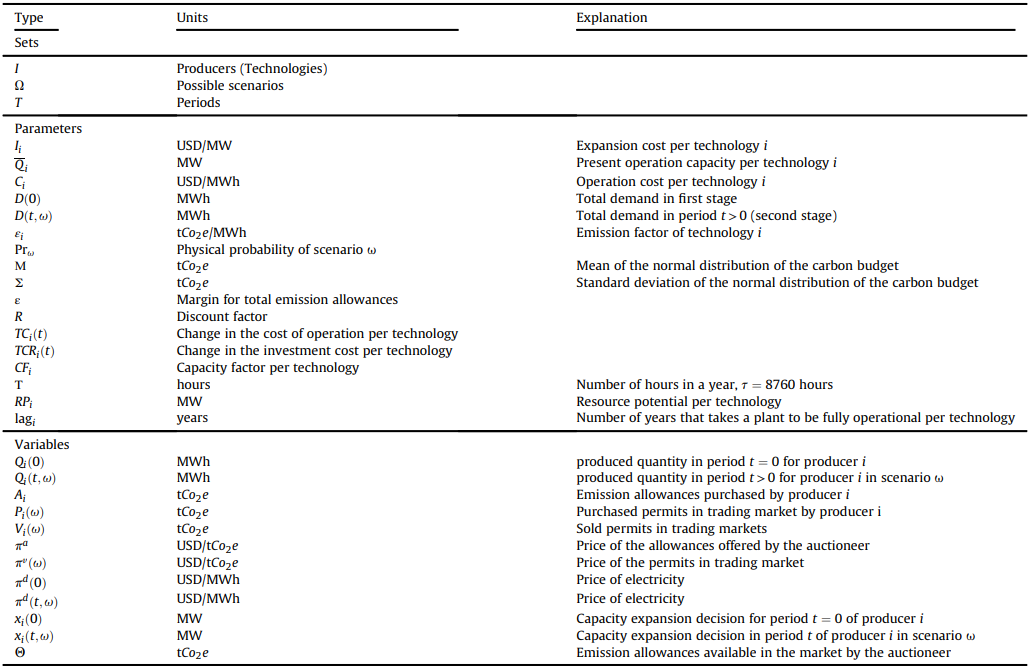
\includegraphics[width=17cm]{Samuel/Memoria Samuel/Imagenes/Tabla amigo.png}
    \caption{Nomenclatura modelo original (Fuente: \protect\citeB{amigo_two_2021})}
    \label{fig:Tabla1}
\end{figure}

\section{Parámetros función del productor: Amigo, Cea-Echenique \& Feijoo (2021)}\label{c25}

Como ya vimos entonces en \ref{c24}, los productores se enfrentan a la tarea de ajustar sus niveles de generación de energía y su inversión en permisos de emisión en respuesta a la demanda revelada. Estos deben tomar la decisión sobre cuánta energía generar y cuántos permisos de emisión comprar o vender, teniendo en cuenta la demanda revelada y los precios de los permisos de emisión.
\vspace{2.5mm}

 Cada productor $i$ representa una única tecnología en la economía (ver Sección ...). El conjunto de variables del productor $i$ en un horizonte temporal de $\bar{t}$ años se compone de: 
 \begin{enumerate}

\item 
Una cantidad de expansión de capacidad $x_i:=\left(x_i(0),(x_i(t,\omega)){(t,\omega)\in T\times\Omega}\right)\in\mathbb{R}+\times\mathbb{R}+^{T\times\Omega}$
 \item 
 Un plan de producción $Q_i:=\left(Q{i}(0),(Q_{i}(t,\omega){(t,\omega)\in T\times\Omega})\right)\in\mathbb{R}+\times\mathbb{R}+^{T\times\Omega}$
 \item 
 Asignaciones de emisiones $A_i\in\mathbb{R}+$ compradas en el primer período $t=0$
 \item 
 Permisos $P_i(\omega)\in\mathbb{R}+^{\Omega}$ comprados en $t=1$ para el intervalo de tiempo $t\in[1,\bar{t}]$
 \item 
 Permisos $V_i(\omega)\in\mathbb{R}+^{\Omega}$ vendidos en $t=1$ para el intervalo de tiempo $t\in[1,\bar{t}]$.

\end{enumerate}
El modelo se ejecuta en intervalos de un año, por lo tanto, representamos el año en bloques de $\tau=8760$ horas. Para cada tecnología, consideramos un factor de capacidad $CF_i\in\mathbb{R}_+$ que representa la operación real de cada planta.
\vspace{2.5mm}

El objetivo de los productores es minimizar el costo. Por lo tanto, para un productor representativo, hay un costo de producción para cada período $t\in T$. Definimos la función de ingresos dada por los precios de la electricidad $\pi^d:=\left(\pi^d(0),\left(\pi^d(t,\omega)\right){(t,\omega)\in T\times\Omega}\right)\in\mathbb{R}+\times\mathbb{R}+^{T\times\Omega}$ (denotada como $p$ en la forma general descrita en la ecuación \ref{eq:revenew}) y los parámetros $(a_i,b_i){i\in{1,...N}}\in(\mathbb{R}^2_+)^N$ como

\begin{align}\label{eq:revenew}
f_i(p,q)=\Big(a_i\cdot q+\frac{b_i}{2}\cdot q^{2}\Big)-p\cdot q.
\end{align}
\vspace{2.5mm}

Definiendo $T_0:={0}\cup T$, el problema de optimización del productor $i$ se formula eligiendo \linebreak$(x_i,Q_i, A_i,P_i,V_i)\in\mathbb{X}:=\left(\mathbb{R}_+\times\mathbb{R}_+^{T\times\Omega}\right) \times\left(\mathbb{R}_+\times\mathbb{R}_+^{T\times\Omega}\right) \times \mathbb{R}_+\times\mathbb{R}_+^{\Omega}\times\mathbb{R}_+^{\Omega}$ dados los precios \linebreak$(\pi^d$, $\pi^a$ , $\pi^v)\in\Pi:=\left(\mathbb{R}_+\times\mathbb{R}_+^{T\times\Omega}\right)\times\mathbb{R}_+\times\mathbb{R}^{\Omega}_+$ , los parámetros \linebreak$\left((a_i,b_i),I_i, TC_i(t,\omega), TCR_i(t,\omega), CF_i,\bar{Q}_i, RP_i , \varepsilon_i\right)\in \Xi:=\mathbb{R}_+^2\times\mathbb{R}_+^7$, $\tau\in \mathbb{R}_+$ y la probabilidad $(Pr(\omega))_{\omega\in\Omega}\in\Delta:=\left\{\left(Pr(\omega)\right)_{\omega\in\Omega}\in[0,1]^K:\sum_{\omega\in\Omega}Pr(\omega)=1\right\}$ como una solución de la ecuación del problema de los productores \ref{fo:prod}. Además este va a estar sujeto a distintas restricciones; de capacidad en generación en la restricción \ref{res:1}, restricción en generación inicial en \ref{res:2}, de límites en capacidad en \ref{res:3} y venta y compra de permisos en \ref{res:4} y \ref{res:5}.


\begin{align}
\min_{(x_i,Q_i,A_i,P_i,V_i)\in \mathbb{X}} & f_i \big( \pi^d(0),Q_i(0)\big)+ A_i \pi^{a} + I_i x_i(0) \nonumber \\ 
& + \sum_{\omega} Pr(\omega)   \Bigg[ \sum_{t>0} \frac{1}{(1+R)^t} \Big[ TC_i(t,\omega)\cdot f_i \big( \pi^d(t,\omega),Q_i(t,\omega) \big) \nonumber \\
& + TCR_i(t,\omega) \cdot I_i\cdot x_i(t,\omega) \Big] + \pi^v(\omega)\cdot \big(P_i(\omega)-V_i(\omega)\big) \Bigg] \label{fo:prod} \\
\textrm{s.a. \ } \nonumber
\end{align}
\begin{align}
\Big(CF_i \cdot\tau\Big)  \Bigg[\bar{Q}_i + \sum_{t^{\prime}<\bar{t}} x_i(t^\prime,\omega) + x_i(0)+ \bar{Q}_i(t) \Bigg] - Q_i(t,\omega) & \geq 0  & \forall  \quad i,\omega, t  > 0 & \quad (\alpha_{i,\omega,t})\label{res:1} \\
\Big(CF_i\cdot\tau \Big)\bar{Q_i}-Q_{i}(0) & \geq 0  & \forall  \quad i & \quad (\kappa_i) \label{res:2} \\
RP_i - \bar{Q}_i  - x_i(0) - \sum_{t > 0} x_i(t,\omega) & \geq 0 &  \forall \quad i,\omega &   \quad (\psi_{i,\omega}) \label{res:3} \\
A_{i} -V_i(\omega) & \geq  0  & \forall  \quad \omega & \quad (\beta_{i,\omega}) \label{res:4} \\
A_{i} + (P_i(\omega) - V_i(\omega))-\sum_{t>0}Q_i(t, \omega)\cdot \varepsilon_{i}-Q_i(0)\varepsilon_{i} & \geq  0  &\forall \quad \omega & \quad (\gamma_{i,\omega})\label{res:5} \\
Q_i(0) & \geq  0 & \forall \quad i & \quad (\lambda_i) \label{res:q0} \\ 
Q_i(t, \omega) & \geq  0   & \forall \quad \omega, t >0 & \quad (\delta_{i,\omega,t})\label{res:qt} \\
x_i(0) & \geq  0 & \forall  \quad i & \quad (\xi_i)  \label{res:capi0} \\ 
x_i(t, \omega) & \geq  0   & \forall  \quad \omega, t >0 & \quad (\varphi_{i,\omega,t})\label{res:capt}
\end{align}


El modelo de \citeB{amigo_two_2021} utiliza una serie de parámetros en su función del productor\ref{fo:prod}. Aquí se presenta una descripción de los más relevantes que se podrían considerar para evaluar la viabilidad económica de la transición hacia combustibles renovables:
\begin{enumerate}

\item 
$I_i$(USD/MW): Costo de expansión por tecnología i. Este parámetro es crucial para evaluar los costos de inversión necesarios para aumentar la capacidad de producción de una tecnología de energía específica.
\item 
$Q_i$(MW): Capacidad de operación actual por tecnología i. Este variable permite evaluar la capacidad de producción actual de diferentes tecnologías de energía.
\item 
$C_i$(USD/MWh): Costo de operación por tecnología i. Este parámetro es esencial para entender los costos operativos asociados con cada tecnología de energía.
\item 

$\varepsilon_{i}$ (tCO2e/MWh): Factor de emisión de la tecnología i. Este parámetro permite cuantificar las emisiones de CO2 asociadas con cada tecnología de energía, lo cual es crucial para evaluar el impacto ambiental de la transición hacia combustibles renovables.
\item 
$TC_i(t)$: Cambio en el costo de operación por tecnología. Este parámetro permite evaluar cómo los costos operativos de una tecnología de energía específica podrían cambiar con el tiempo.
\item 
$TCR_i(t)$: Cambio en el costo de inversión por tecnología. Este parámetro permite evaluar cómo los costos de inversión de una tecnología de energía específica podrían cambiar con el tiempo.
\item 
$CF_i$: Factor de capacidad por tecnología. Este parámetro permite evaluar la eficiencia de diferentes tecnologías de energía.
\item 
$RP_i$ (MW): Potencial de recurso por tecnología. Este parámetro permite evaluar el potencial de producción de diferentes tecnologías de energía.
\end{enumerate}

Estos parámetros van a permitir evaluar tanto los costos económicos como los impactos ambientales de la transición hacia combustibles renovables.





